\chapter{Background and related work}
\thispagestyle{main} % Needed for Footer and Header on Chapterpage
The following section either introduces the tools and technologies used in bazo or references explanations of previous theses in the context of the bazo-blockchain. Also the theses of other students working on the bazo-blockchain are referenced.
\pagebreak

\section{Related work}
At the time of writing the thesis the bazo-blockchain contains the software systems as described in the following system context diagram \ref{systemcontextdiagram}. There are also some smaller tools which are not further described. In \ref{systemcontextdiagram} multiple miner instances are displayed to represent the blockchain and to describe how the miner interact with eachother.

\vfill

\begin{figure}[H]
	\begin{center}
	\includegraphics[width=\textwidth]{./images/BAZO_System_Context}
	\caption{BAZO blockchain system context diagram}
	\label{systemcontextdiagram}
	\end{center}
\end{figure}
\pagebreak

The bazo-blockchain currently contains the following sub projects:
\begin{description}
  \item[Miner] The miner is at the heart of the blockchain. It validates transactions, keeps the ledger up to date and contacts other miners about new transactions or blocks.
  \item[Wallet] 
  \item[Virtual machine] The virtual machine executes the code of the contract.
  \item[Client] The client is used to create and send new transactions.
  \item[Block explorer] The block explorer is used to view transactions.
\end{description}


There are also some further small useful tools, liky keygen but they are not further discussed here. The organization on github is accessible under the following link: \href{https://github.com/bazo-blockchain}{https://github.com/bazo-blockchain}.

In the \ref{systemcontainerdiagram} one of the miners is expanded which makes it possible to see it's packages and their relationships with other components.
\begin{figure}[H]
	\begin{center}
	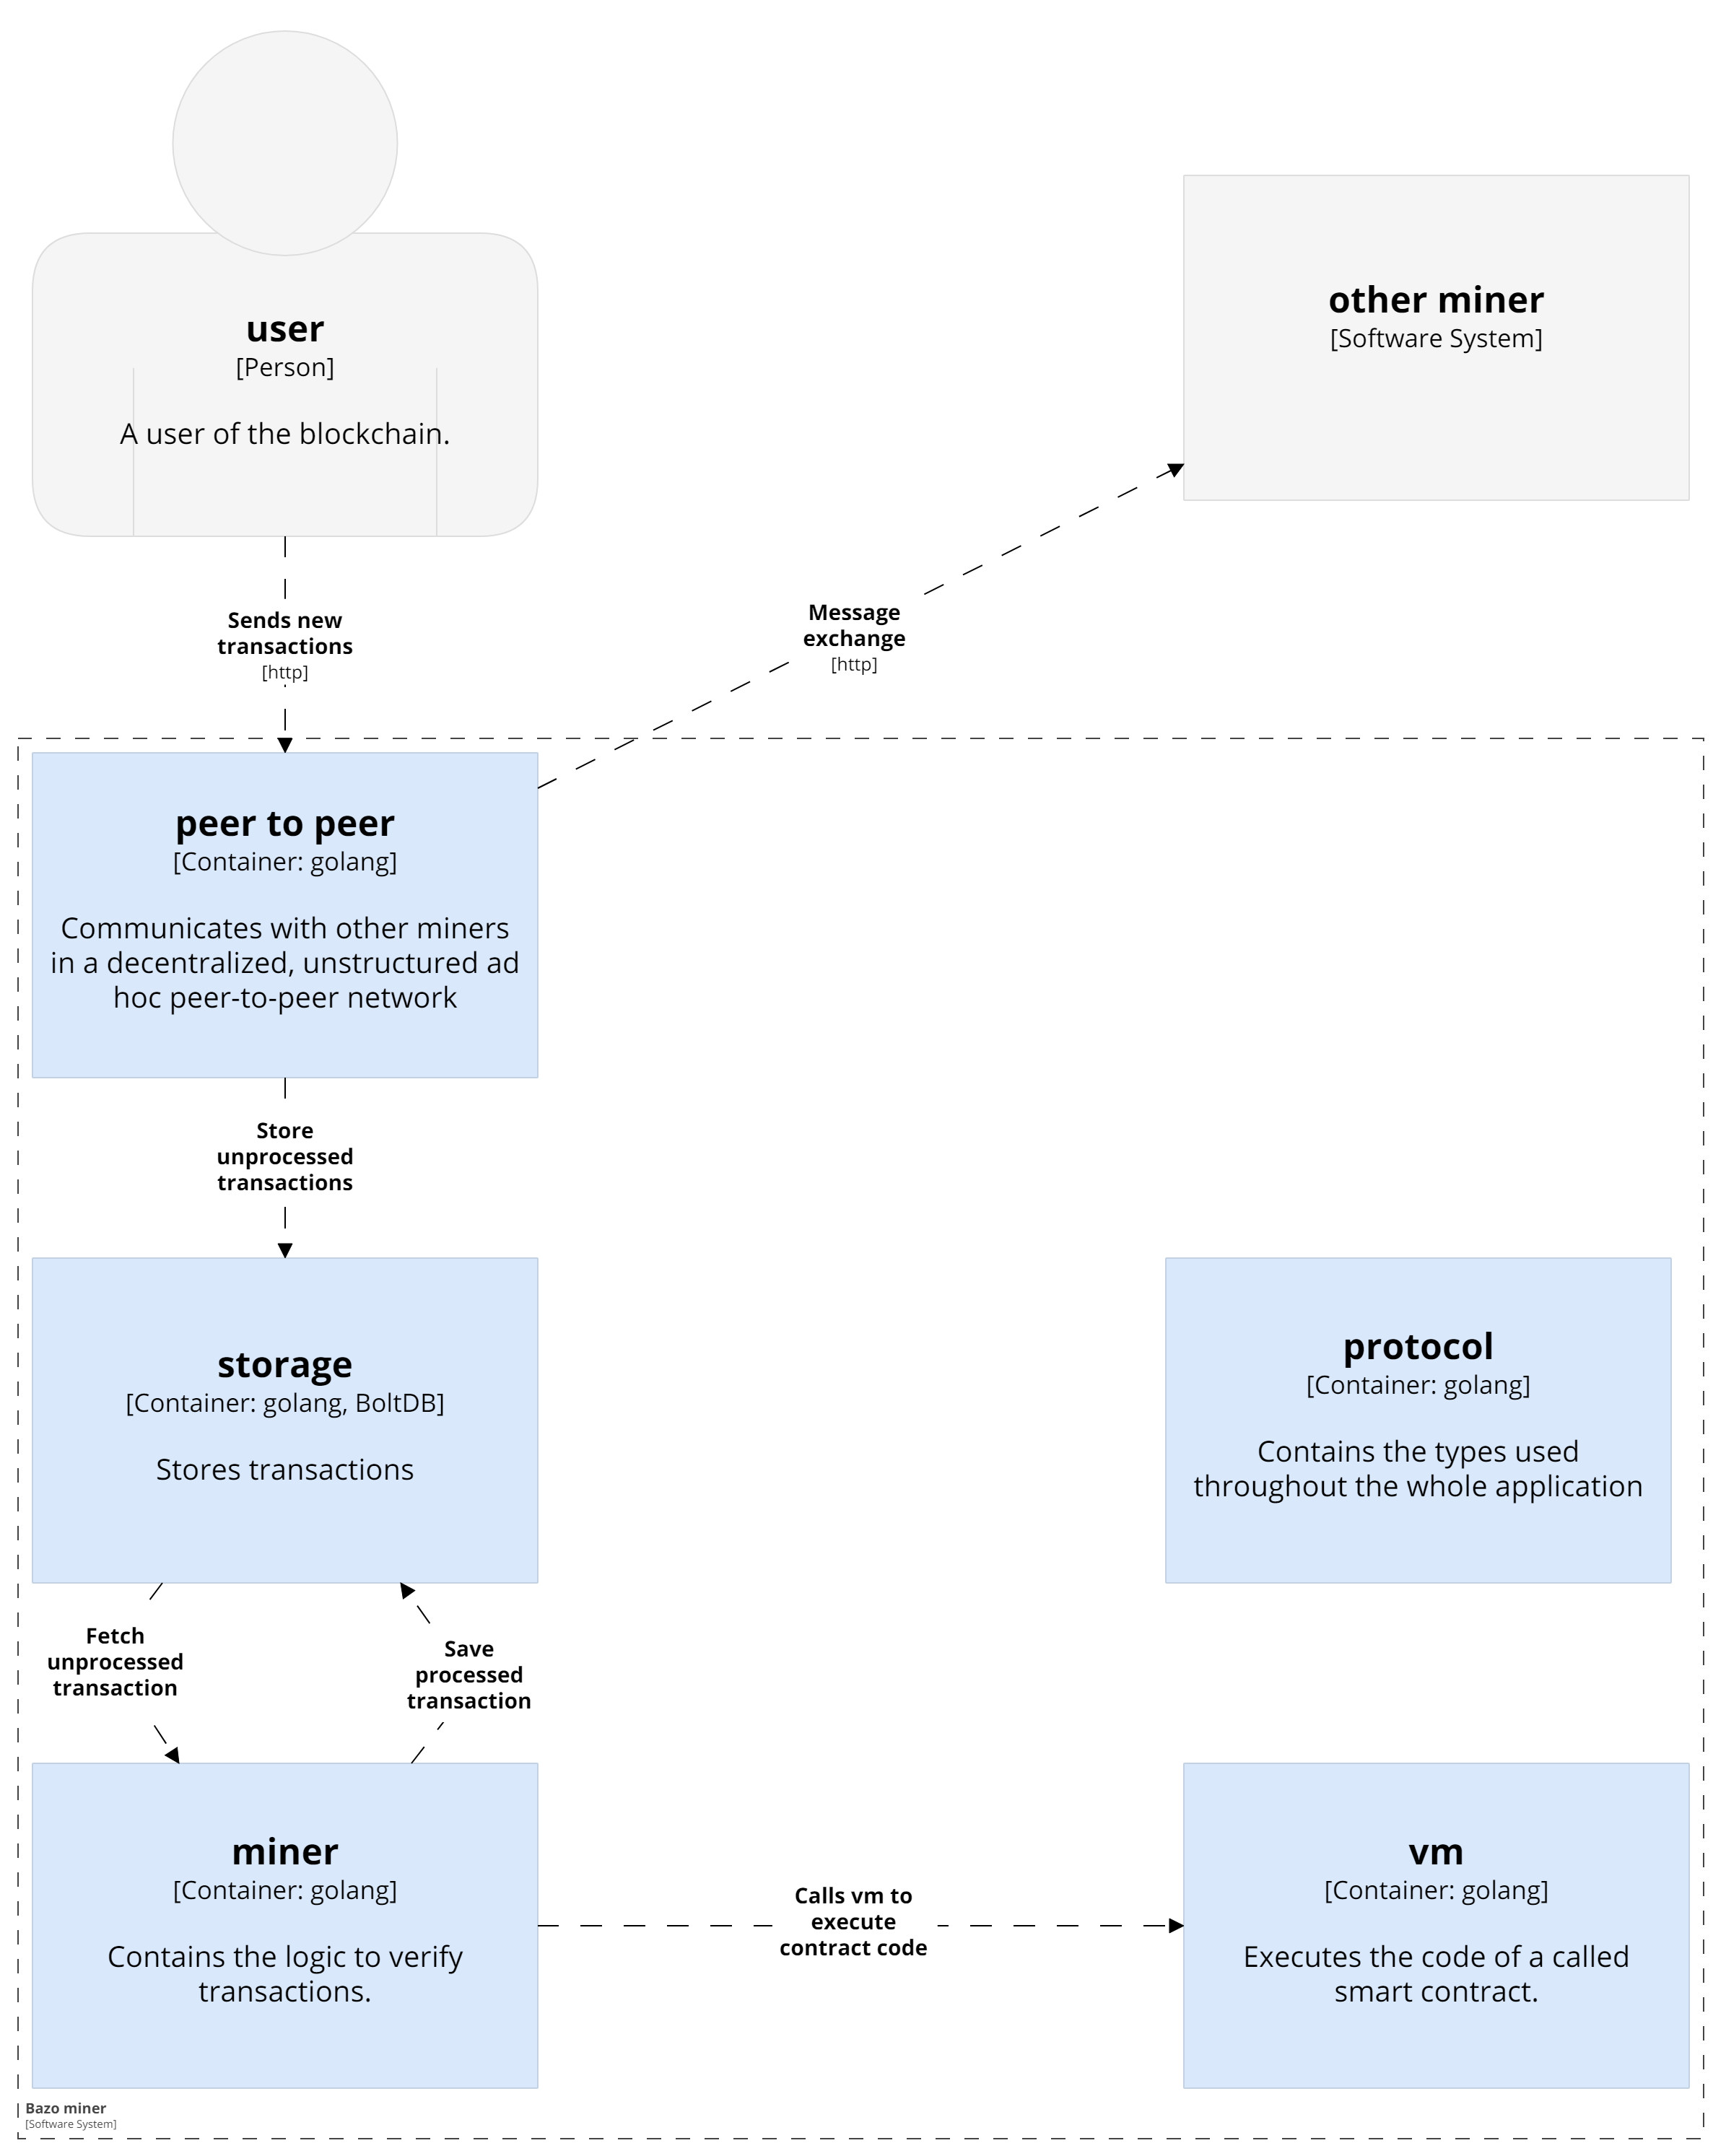
\includegraphics[width=\textwidth]{./images/BAZO_Container}
	\caption{BAZO blockchain container diagram}
	\label{systemcontainerdiagram}
	\end{center}
\end{figure}
\pagebreak

\subsection{Previous work}
As the BAZO blockchain was started in 2017 there have been multiple theses within which different aspects of the blockchain were implemented. 
\begin{itemize}
	\item Bazo – A Cryptocurrency from Scratch \cite{ba_miner}
	\item A Progressive Web App (PWA)-based Mobile Wallet for Bazo \cite{ba_wallet}
	\item A Blockchain Explorer for Bazo \cite{ba_explorer}
	\item Proof of Stake for Bazo \cite{ba_pos}
	\item Design and Prototypical Implementation of a Mobile Light Client for the Bazo Blockchain \cite{ba_client}
\end{itemize}

\subsection{Similar existent projects}
A huge help in being able to reason by analogy were the open source repositories of NEO and Ethereum. We learned a lot by looking through their code while building our own VM. Basically all three (BAZO, Ethereum and NEO) are platforms for decentralized applications on the basis of smart contracts. 

\subsubsection{NEO}
NEO is a blockchain project \frqq that utilizes blockchain technology and digital identity to digitize assets, to automate the management of digital assets using smart contracts, and to realize a smart economy with a distributed network.\frqq \cite{neovseth}

\subsubsection{Ethereum}
The goal of Ethereum is to create a platform for the development of decentralized apps in order to create a \frqq more globally accessible, more free, and more trustworthy Internet, an internet 3.0\frqq. \cite{neovseth}

\subsubsection{How do they differ from the Bazo Blockchain?}
As for now, Bazo is just a research project but the goal is also to become a platform for Decentralized Applications but for that a dedicated team would be needed. 
\pagebreak

\section{Background}
In this section the tools and technologies used to build the bazo-blockchain are explained.

\subsection{Blockchain}
What is a blockchain and reference livios work for blockchain based cryptocurrencies. Blockchains are basically blocks of data chained together by hashfunctions. The data inside these blocks are transactions. In order to make the non-repudiatable digital signatures are used. The transactions are also validated by a miner. The miner validates the signatures and checks if the assed transmitted by the transaction, usually money actually exists on the account of the other person. Since the bazo-blockchain is also account based, it also updates the balance of the account according to the transmitted value. Previous theses in the context of bazo also dive deeper into cryptocurrencies and blockchains [BA lsige, MA chetelat].

Write that bazo blockchain is an account based blockchain.

\subsection{Smart contracts}
A smart contract is basically an agreement or contract written in computer code, saved in a transaction and therefore distributed over the whole network. The smart contract can then be called by another transaction an is executed by the miner. 

\subsection{Transactions}
In the context of data base management systems a transaction is a unit of work performed within the system. \cite{dbtransaction} This definition is also applicable for blockchains. As explained in \autoref{sec:transactionTypes}
there are multiple transaction types and only some are used to send coins. Others are used mostly to change the system state or create a new account.

\subsection{Virtual machine}
A virtual machine in the context of one process is an abstraction layer which abstracts the formulation of the problem from the code that is actually run on a machine in order to make the formulation platform independent.